\documentclass[11pt,a4paper]{article}
\usepackage{isabelle,isabellesym}
\usepackage{fullpage}
\usepackage[usenames,dvipsnames]{color}
\usepackage{document}

% further packages required for unusual symbols (see also
% isabellesym.sty), use only when needed

\usepackage{amssymb}
  %for \<leadsto>, \<box>, \<diamond>, \<sqsupset>, \<mho>, \<Join>,
  %\<lhd>, \<lesssim>, \<greatersim>, \<lessapprox>, \<greaterapprox>,
  %\<triangleq>, \<yen>, \<lozenge>

\usepackage[english]{babel}
  %option greek for \<euro>
  %option english (default language) for \<guillemotleft>, \<guillemotright>

\usepackage{stmaryrd}
  %for \<Sqinter>

\usepackage{eufrak}
  %for \<AA> ... \<ZZ>, \<aa> ... \<zz> (also included in amssymb)

%\usepackage{textcomp}
  %for \<onequarter>, \<onehalf>, \<threequarters>, \<degree>, \<cent>,
  %\<currency>

% this should be the last package used
\usepackage{pdfsetup}

\usepackage{graphicx}

\usepackage{url}

% urls in roman style, theory text in math-similar italics
\urlstyle{rm}
\isabellestyle{it}

% for uniform font size
%\renewcommand{\isastyle}{\isastyleminor}

\begin{document}

\title{Isabelle/UTP: Mechanised Theory Engineering for \\ Unifying Theories of Programming}

\author{Simon Foster\footnote{Department of Computer Science, University of York. \href{mailto:simon.foster@york.ac.uk}{simon.foster@york.ac.uk}}, Frank Zeyda, Yakoub Nemouchi, Pedro Ribeiro, and Burkhart Wolff}

\maketitle

\begin{abstract}
  Isabelle/UTP is a mechanised theory engineering toolkit based on Hoare and He's Unifying Theories of Programming
  (UTP). UTP enables the creation of denotational, algebraic, and operational semantics for different programming
  languages using an alphabetised relational calculus. We provide a semantic embedding of the alphabetised relational
  calculus in Isabelle/HOL, including new type definitions, relational constructors, automated proof tactics, and
  accompanying algebraic laws. Isabelle/UTP can be used to both capture laws of programming for different languages, and
  put these fundamental theorems to work in the creation of associated verification tools, using calculi like Hoare
  logics. This document describes the relational core of the UTP in Isabelle/HOL.
\end{abstract}

\tableofcontents

\begin{center}
  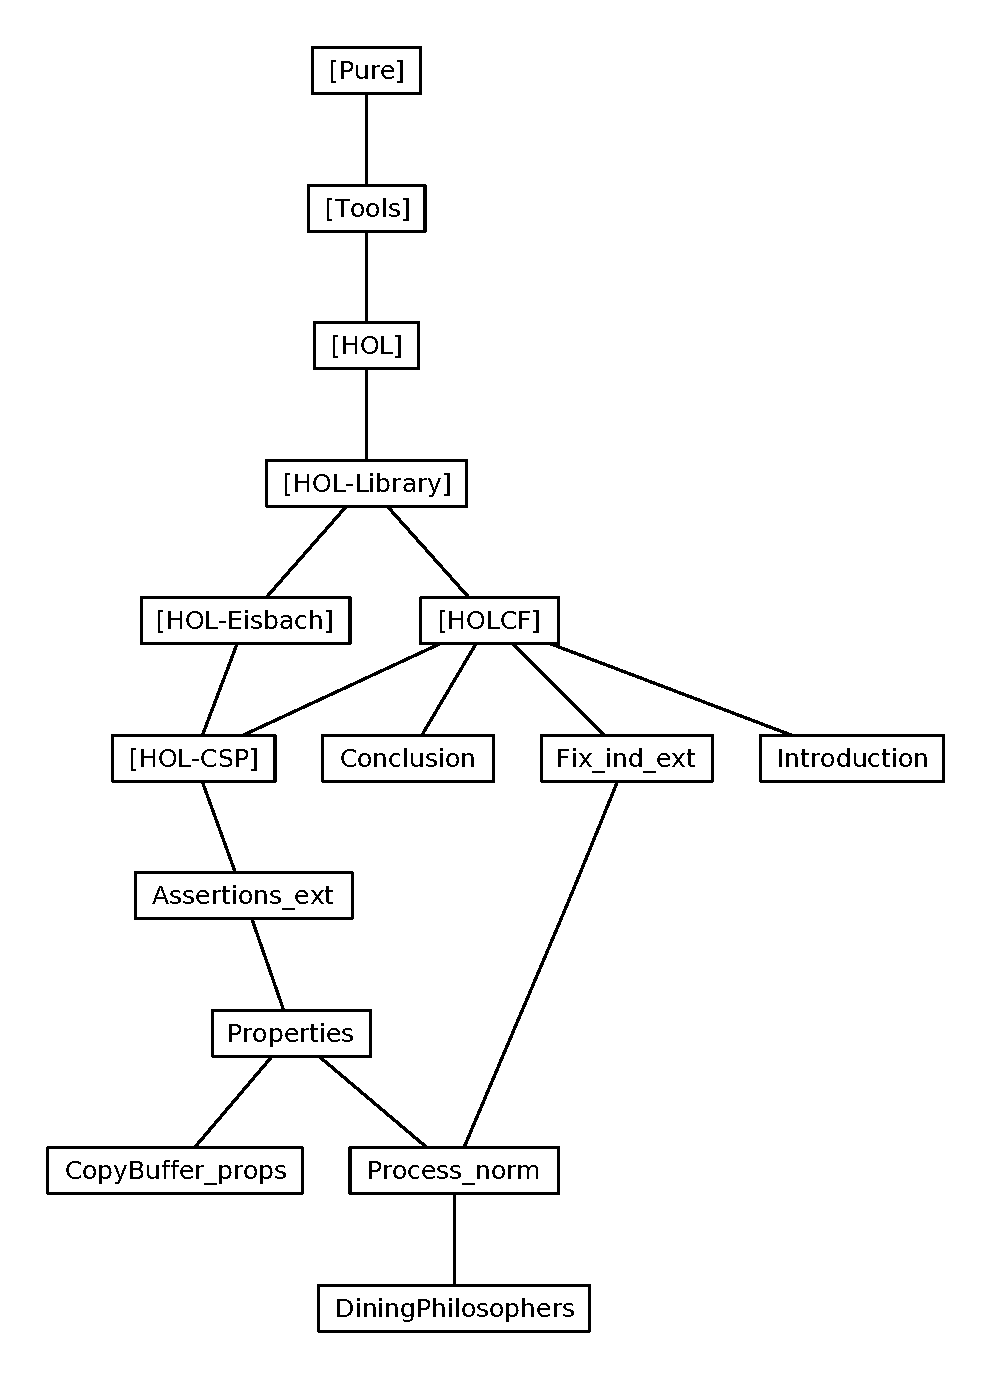
\includegraphics[height=\textheight]{session_graph}
\end{center}

% sane default for proof documents
\parindent 0pt\parskip 0.5ex

\section{Introduction}

This document contains the description of our mechanisation of Hoare and He's \emph{Unifying Theories of
  Programming}~\cite{Hoare&98,Cavalcanti&06} (UTP) in Isabelle/HOL. UTP uses the ``programs-as-predicates'' approach, 
pioneered by Hehner~\cite{Hehner1988,Hehner1990,Hehner93}, to encode denotational semantics and facilitate reasoning about programs. 
It uses the alphabetised relational calculus, which combines predicate calculus and relation algebra, to denote programs as relations 
between initial variables ($x$) and their subsequent values ($x'$). Isabelle/UTP\footnote{Isabelle/UTP website:
  \url{https://www.cs.york.ac.uk/circus/isabelle-utp/}}~\cite{Foster16a,Foster16c,Foster14c} semantically embeds this
relational calculus into Isabelle/HOL, which enables application of the latter's proof facilities to program
verification. For an introduction to UTP, we recommend two tutorials~\cite{Cavalcanti04,Cavalcanti&06}, and also the UTP
book~\cite{Hoare&98}.

The Isabelle/UTP core mechanises most of definitions and theorems from chapters 1, 2, 4, and 7 of \cite{Hoare&98}, and some material
contained in chapters 5 and 10. This essentially amounts to alphabetised predicate calculus, its core laws, the UTP
theory infrastructure, and also parallel-by-merge~\cite[chapter~5]{Hoare&98}, which adds concurrency primitives. The
Isabelle/UTP core does not contain the theory of designs~\cite{Cavalcanti04} and CSP~\cite{Cavalcanti&06}, which are
both represented in their own theory developments.

A large part of the mechanisation, however, is foundations that enable these core UTP theories. In particular,
Isabelle/UTP builds on our implementation of lenses~\cite{Foster16a,Optics-AFP}, which gives a formal semantics to state
spaces and variables. This, in turn, builds on a previous version of Isabelle/UTP~\cite{Feliachi2010,Feliachi2012},
which provided a shallow embedding of UTP by using Isabelle record types to represent alphabets. We follow this approach
and, additionally, use the lens laws~\cite{Foster09,Foster16a} to characterise well-behaved variables. We also add
meta-logical infrastructure for dealing with free variables and substitution. All this, we believe, adds an additional
layer rigour to the UTP.

The alphabets-as-types approach does impose a number of theoretical limitations. For example, alphabets can only be
extended when an injection into a larger state-space type can be exhibited. It is therefore not possible to arbitrarily
augment an alphabet with additional variables, but new types must be created to do this. This is largely because
as in previous work~\cite{Feliachi2010,Feliachi2012}, we actually encode state spaces rather than alphabets, 
the latter being implicit. Namely, a relation is typed by the state space type that it manipulates, and the alphabet
is represented by collection of lenses into this state space. This aspect of our mechanisation is actually much closer 
to the relational program model in Back's refinement calculus~\cite{Back1998}. 

The pay-off is that the Isabelle/HOL type checker can be directly applied to relational constructions, which makes proof much more automated and
efficient. Moreover, our use of lenses mitigates the limitations by providing meta-logical style operators, such as
equality on variables, and alphabet membership~\cite{Foster16a}. Isabelle/UTP can therefore directly
harness proof automation from Isabelle/HOL, which allows its use in building efficient verification
tools~\cite{Foster18a,Foster18b}. For a detailed discussion of semantic embedding approaches, please see~\cite{Foster16c}.

In addition to formalising variables, we also make a number of generalisations to UTP laws. Notably, our lens-based
representation of state leads us to adopt Back's approach to both assignment and local
variables~\cite{Back1998}. Assignment becomes a point-free operator that acts on state-space update functions, which
provides a rich set of algebraic theorems. Local variables are represented using stacks, unlike in the UTP book where
they utilise alphabet extension.

\pagebreak

We give a summary of the main contributions within the Isabelle/UTP core, which can all be seen in the table of
contents.

\begin{enumerate}
  \item Formalisation of variables and state-spaces using lenses~\cite{Foster16a};
  \item an expression model, together with lifted operators from HOL;
  \item the meta-logical operators of unrestriction, used-by, substitution, alphabet extrusion, and alphabet restriction;
  \item the alphabetised predicate calculus and associated algebraic laws;
  \item the alphabetised relational calculus and associated algebraic laws;
  \item proof tactics for the above based on interpretation~\cite{Huffman13};
  \item a formalisation of UTP theories using locales~\cite{Ballarin06} and building on HOL-Algebra~\cite{Ballarin17};
  \item Hoare logic~\cite{Hoare1969-Logic} and dynamic logic~\cite{Harel1984-DynamicLogic};
  \item weakest precondition and strongest postcondition calculi~\cite{Dijkstra75};
  \item concurrent programming with parallel-by-merge;
  \item relational operational semantics.
\end{enumerate}

% generated text of all theories
\input{session}

\pagebreak

\section*{Acknowledgements}

This work is funded by the EPSRC projects CyPhyAssure\footnote{CyPhyAssure Project:
  \url{https://www.cs.york.ac.uk/circus/CyPhyAssure/}} (Grant EP/S001190/1), RoboCalc\footnote{RoboCalc Project:
  \url{https://www.cs.york.ac.uk/circus/RoboCalc/}} (Grant EP/M025756/1), and the Royal Academy of Engineering.

% optional bibliography
\bibliographystyle{abbrv}
\bibliography{root}

\end{document}
